\documentclass[]{beamer}

\usepackage[]{graphicx}
%\usepackage[]{minted}
\usepackage[]{enumitem}

\usetheme[]{Madrid}
%\usetheme[]{Dresden}
%\usetheme[]{Antibes}
%\usetheme[]{Boadilla}
\usefonttheme[onlymath]{serif}
\graphicspath{ {./images/} }
\title[]{Attention}
\author{HE Jiayou}
\date{\today}

\usepackage[backend=biber]{biblatex}

\addbibresource{refs.bib}
\setbeamerfont{footnote}{size=\tiny} %reduce the size of the footnote citation
\setbeamertemplate{bibliography item}{\insertbiblabel}  % Add numbered list of references in the end

\newcommand{\bb}[1]{\mathbb{#1}}
\newcommand{\x}{\times}
\newcommand{\vc}[1]{\mathbf{#1}}

\AtBeginSection[]
{
    \begin{frame}<beamer>
        \frametitle{Outline}
        \tableofcontents[
            currentsection,
            subsectionstyle=show/hide,
        ]
    \end{frame}
}

\begin{document}

\frame{\titlepage}

\begin{frame}
    \frametitle{Table of Contents}
    \tableofcontents[subsectionstyle=hide, subsubsectionstyle=hide]
\end{frame}

\section{RNN}
\begin{frame}
    \frametitle{RNN}
    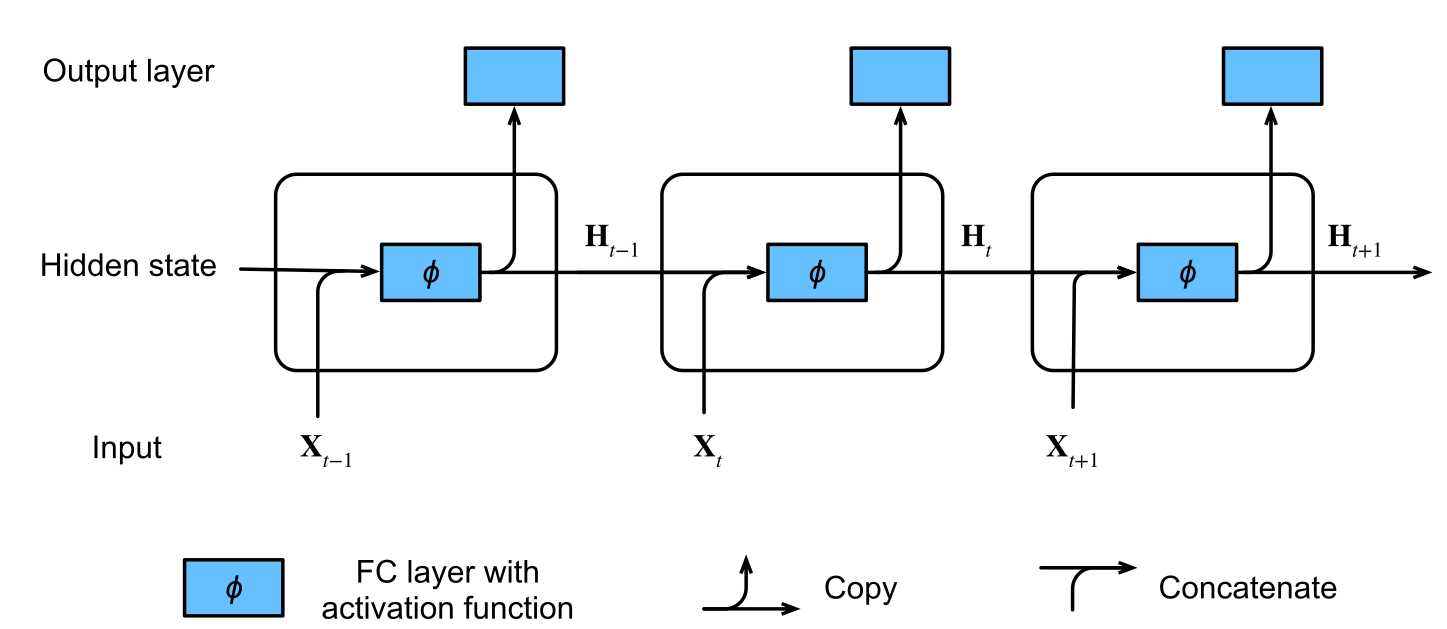
\includegraphics[scale = 0.2]{RNN.png}
    \begin{columns}
        \column{0.5 \textwidth}
        \begin{align*}
            H_t &= \phi\bigl(X_t W_{xh} + H_{t-1}W_{hh} + b_h\bigr) \\
            O_t &= H_t W_{hq} + b_q
        \end{align*}
        \column{0.5 \textwidth}
        \begin{align*}
            &X_t \in \bb{R}^{n\x d}~~H_t \in \bb{R}^{n\x h} \\
            &O_t \in \bb{R}^{n\x q}~~b_h \in \bb{R}^{1\x h} \\
        \end{align*}
    \end{columns}
    \footfullcite[]{D2l}
\end{frame}

\subsection{GRU}
\begin{frame}
    \frametitle{GRU\: Gated Recurrent Unit} 
    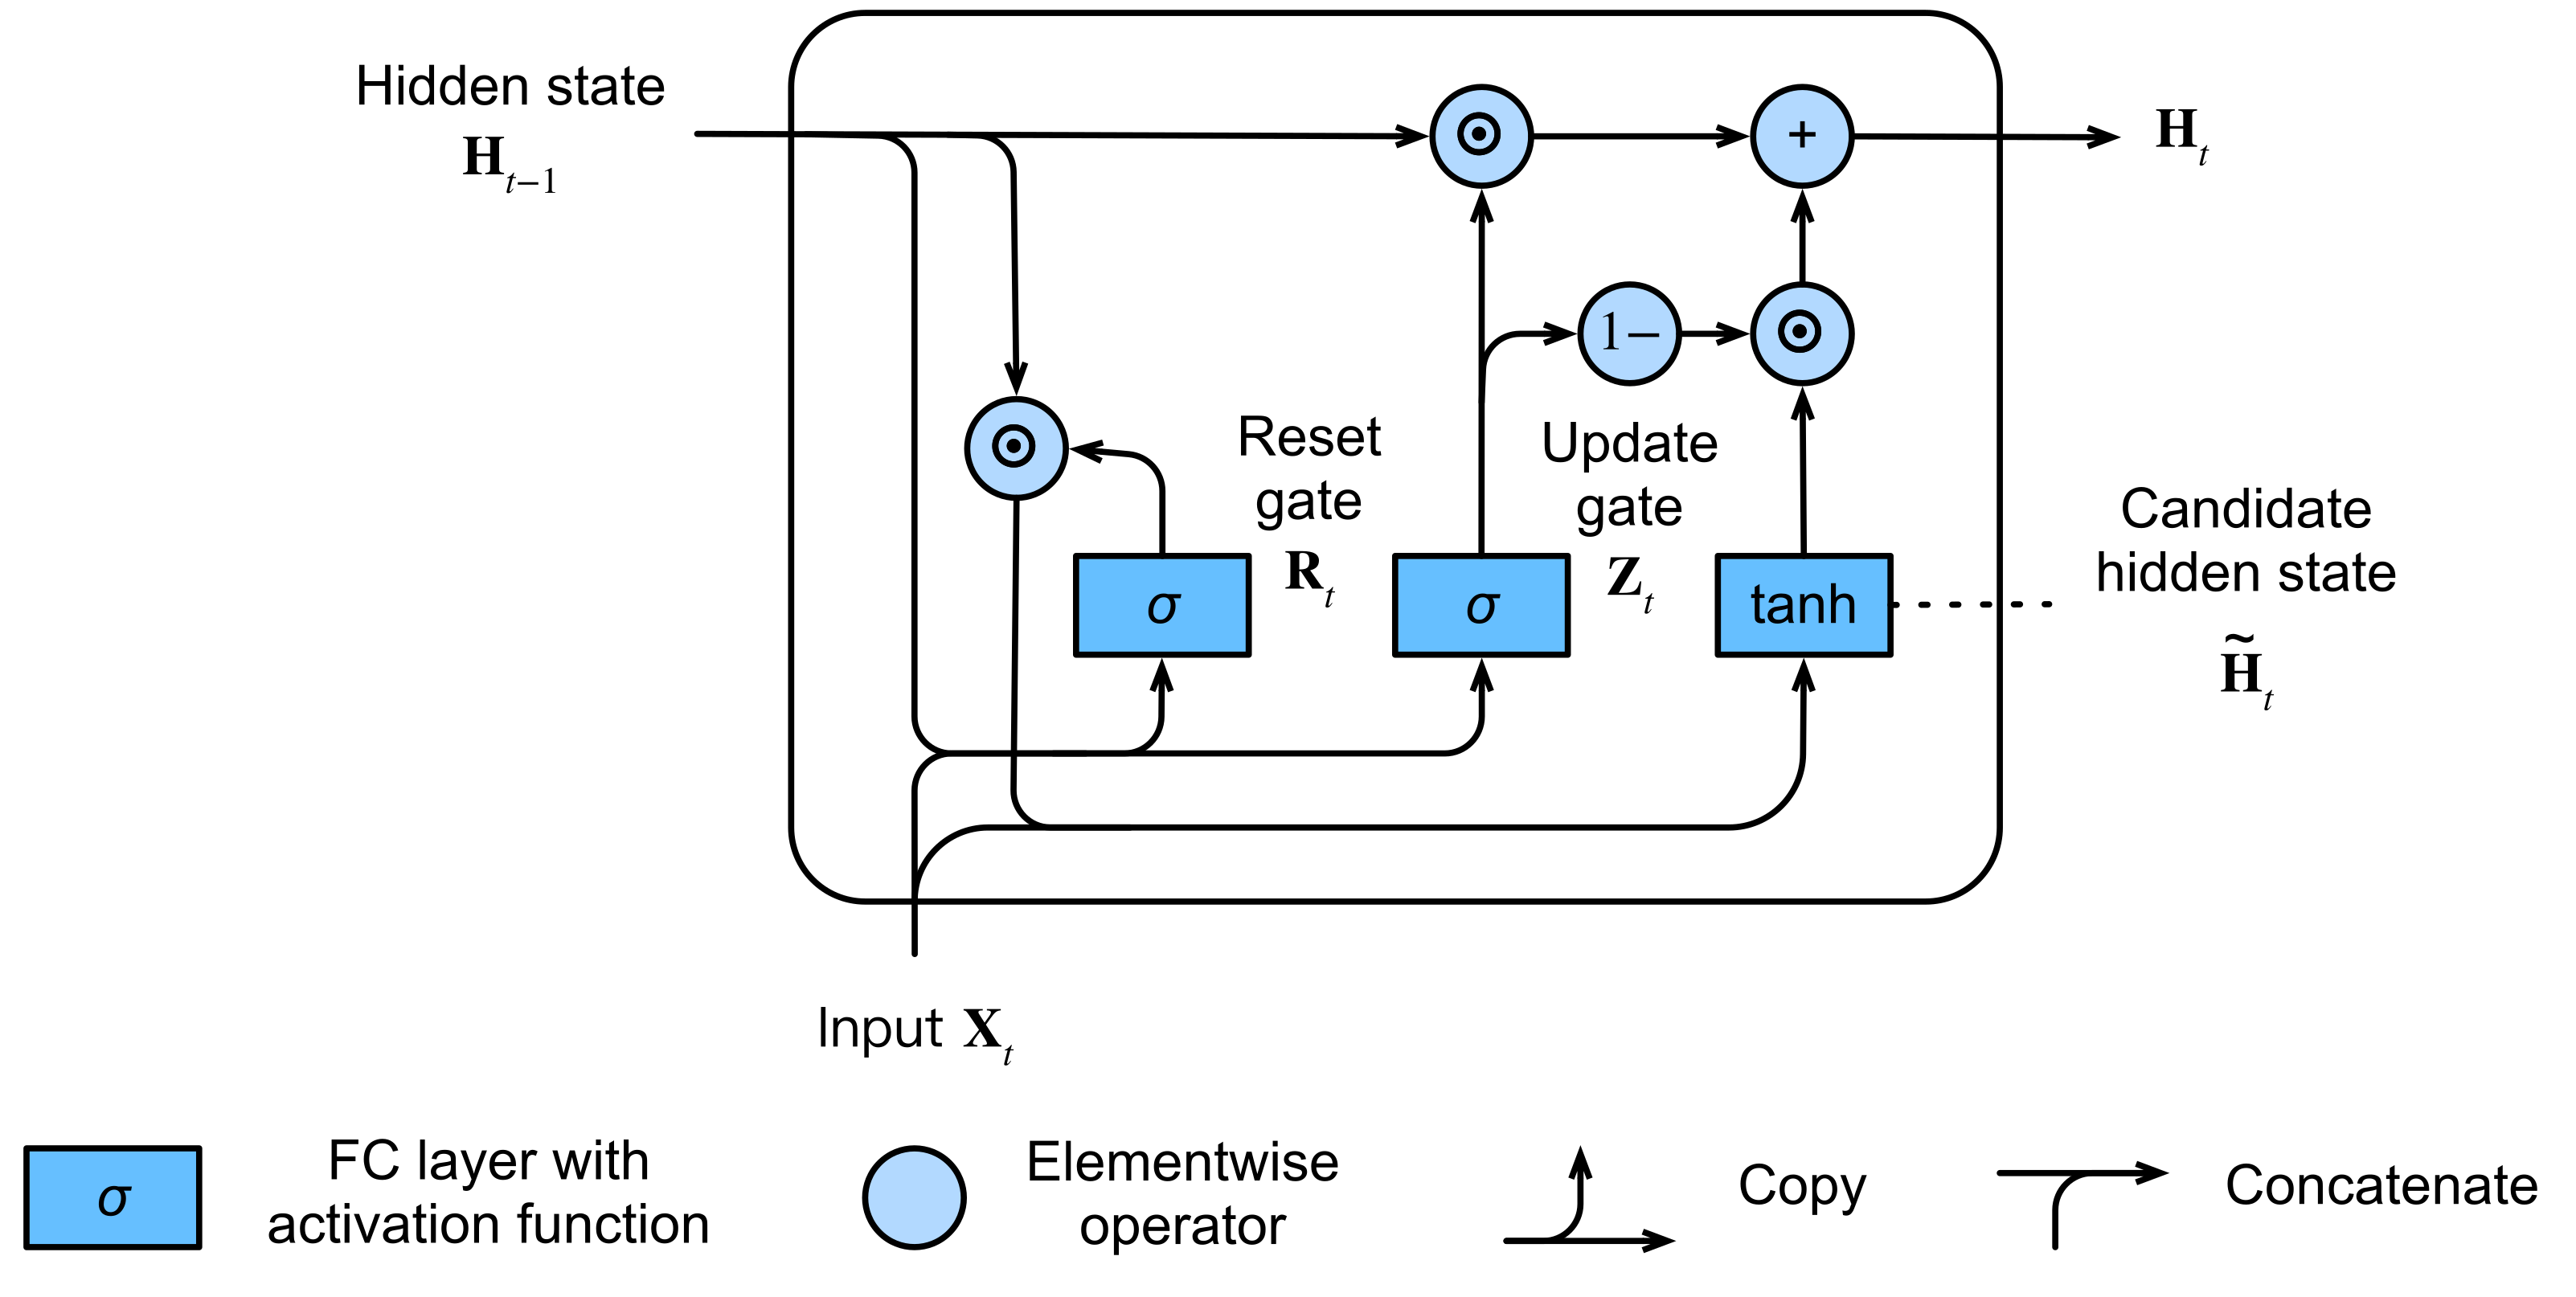
\includegraphics[scale = 0.1]{GRU.png}
\end{frame}
\begin{frame}
    \frametitle{GRU\: Gated Recurrent Unit} 
    GRU supports gating of the hidden state.
    \begin{itemize}[label=\textbullet]
        \item Reset gates help capture short-term dependencies in sequences.
        \item Update gates help capture long-term dependencies in sequences.
    \end{itemize}
    \begin{align*}
        R_t &= \sigma\bigl(X_t W_{xr} + H_{t-1}W_{hr} + b_r\bigr) \\
        Z_t &= \sigma\bigl(X_t W_{xz} + H_{t-1}W_{hz} + b_z\bigr) \\
        \tilde{H_t} &= \tanh \bigl(X_t W_{xh} + \bigl(R_t \odot H_{t-1}\bigr)W_{hh} + b_h\bigr) \\
        H_t &= Z_t \odot H_{t-1} + \bigl(1-Z_t\bigr) \odot \tilde{H_t} 
    \end{align*}
\end{frame}

\subsection{LSTM}
\begin{frame}
    \frametitle{LSTM}
    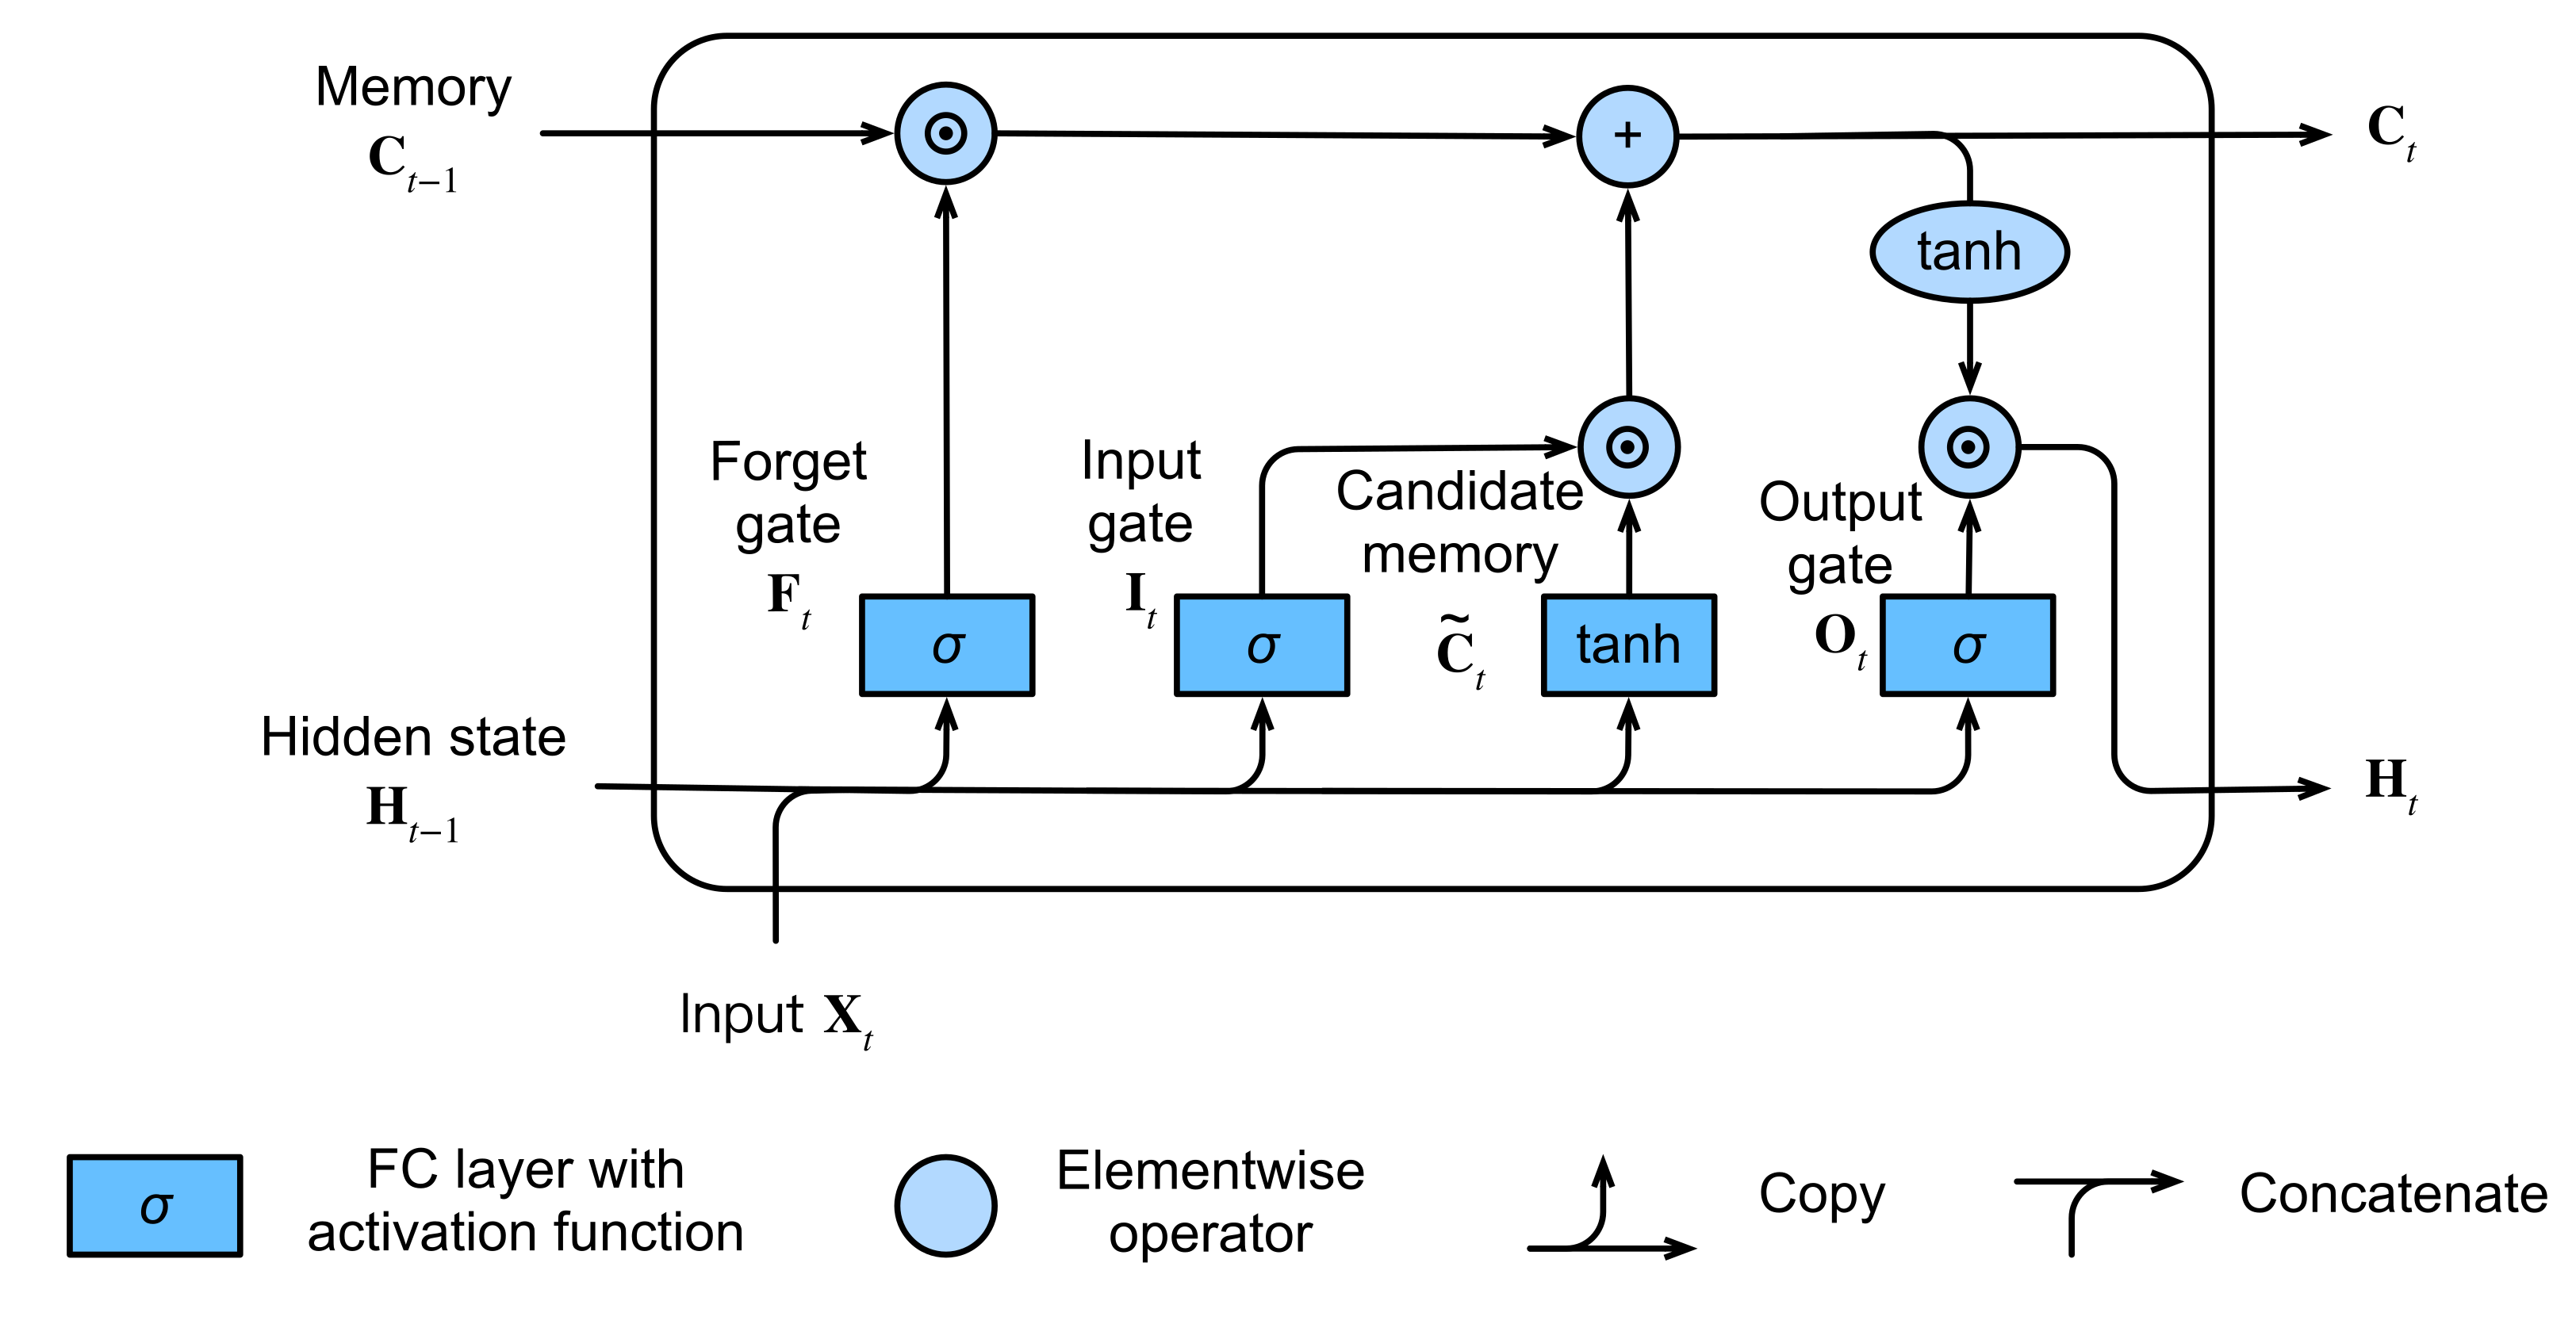
\includegraphics[scale = 0.1]{LSTM.png}
\end{frame}
\begin{frame}
    \frametitle{LSTM}
    The idea is similar to GRU\@.
    \begin{align*}
        I_t &= \sigma\bigl(X_t W_{xi} + H_{t-1} W_{hi} + b_i\bigr) \\
        F_t &= \sigma\bigl(X_t W_{xf} + H_{t-1} W_{hf} + b_f\bigr) \\
        O_t &= \sigma\bigl(X_t W_{xo} + H_{t-1} W_{ho} + b_o\bigr) \\
        \tilde{C_t} &= \tanh \bigl(X_t W_{xc} + H_{t-1}W_{hc} + b_c\bigr) \\
        C_t &= F_t \odot C_{t-1} + I_t \odot \tilde{C_t} \\
        H_t &= O_t \odot \tanh(C_t)
    \end{align*}
\end{frame}

\subsection{Encoder-Decoder}
\begin{frame}
    \frametitle{Encoder-Decoder}
    \begin{figure}
        \centering
        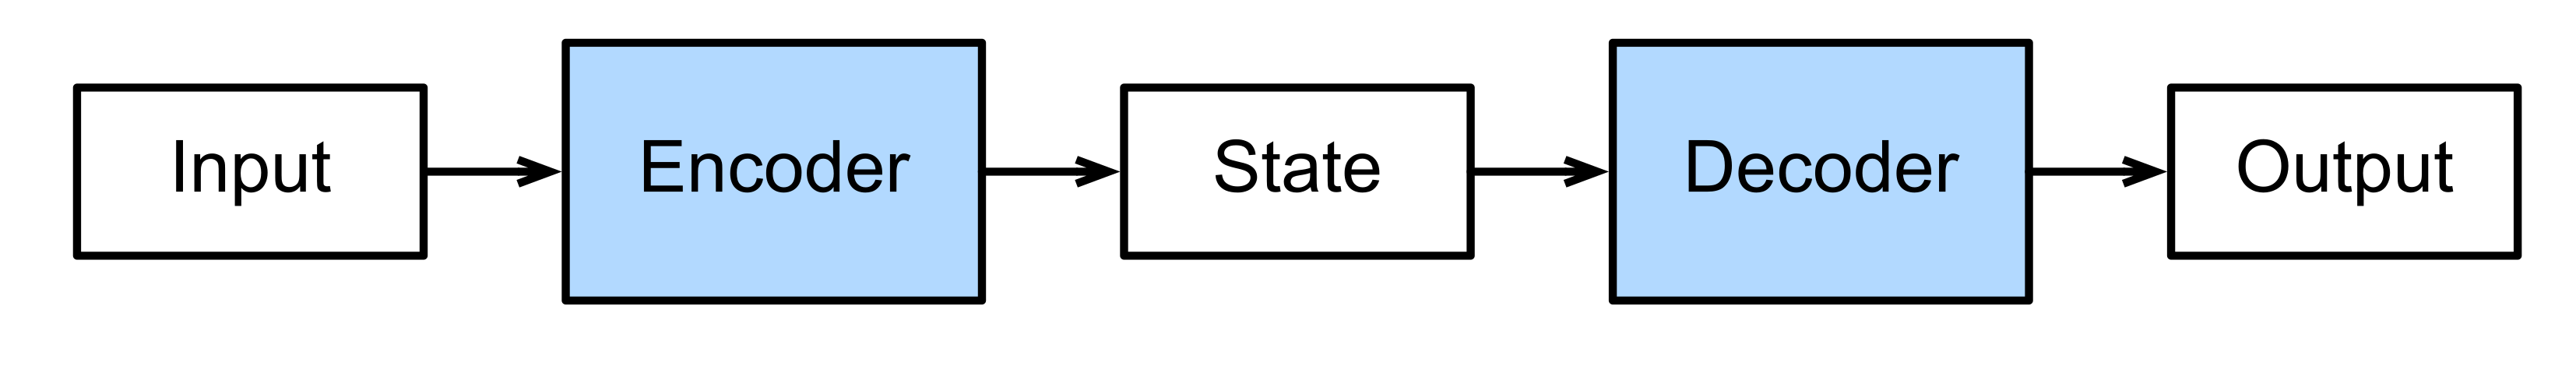
\includegraphics[scale=0.08]{encoder-decoder.png}
        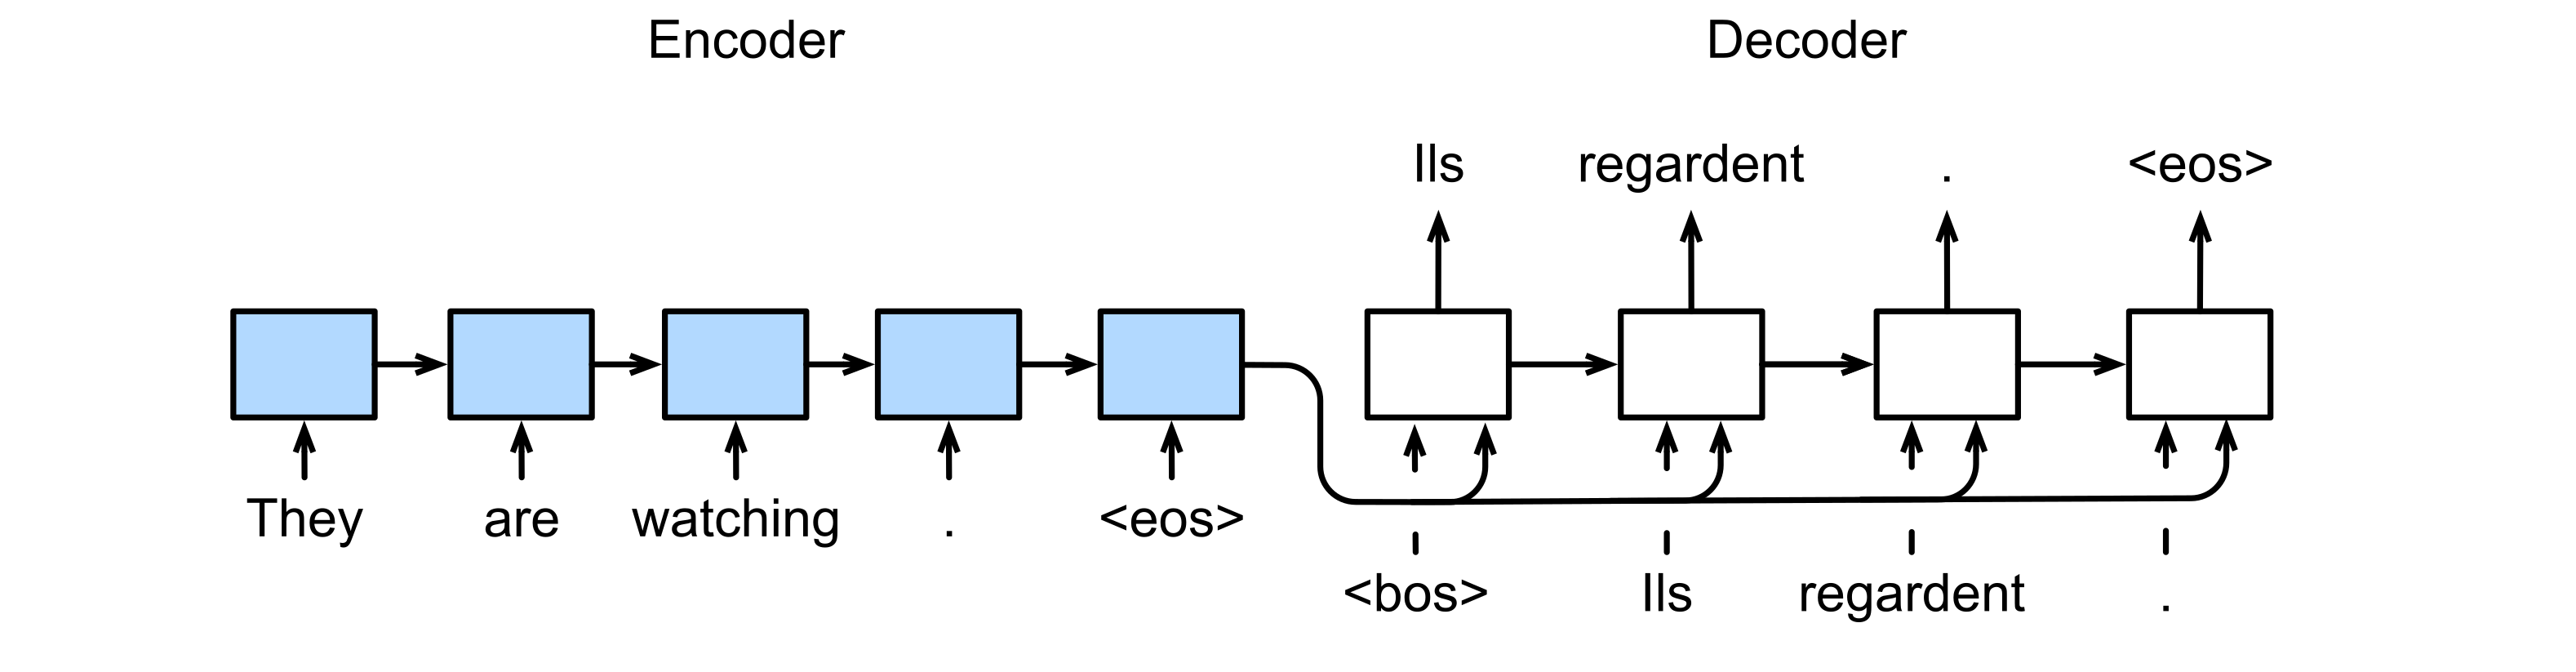
\includegraphics[scale=0.10]{seq2seq.png}
    \end{figure}   
    \centering
\end{frame}
\begin{frame}
    \frametitle{Encoder-Decoder}
    \begin{itemize}[label = \textbullet]
        \item Encoder: $H_t = f\bigl(X_t, H_{t-1}\bigr)$, $C = g\bigl(H_1, \ldots, H_t\bigr)$
        \item Decoder: to get $P(Y_t | Y_1, \ldots, Y_{t-1}, C)$, $H_t = g\bigl(Y_{t-1}, C, H_{t-1}\bigr)$.
    \end{itemize}
    \centering
    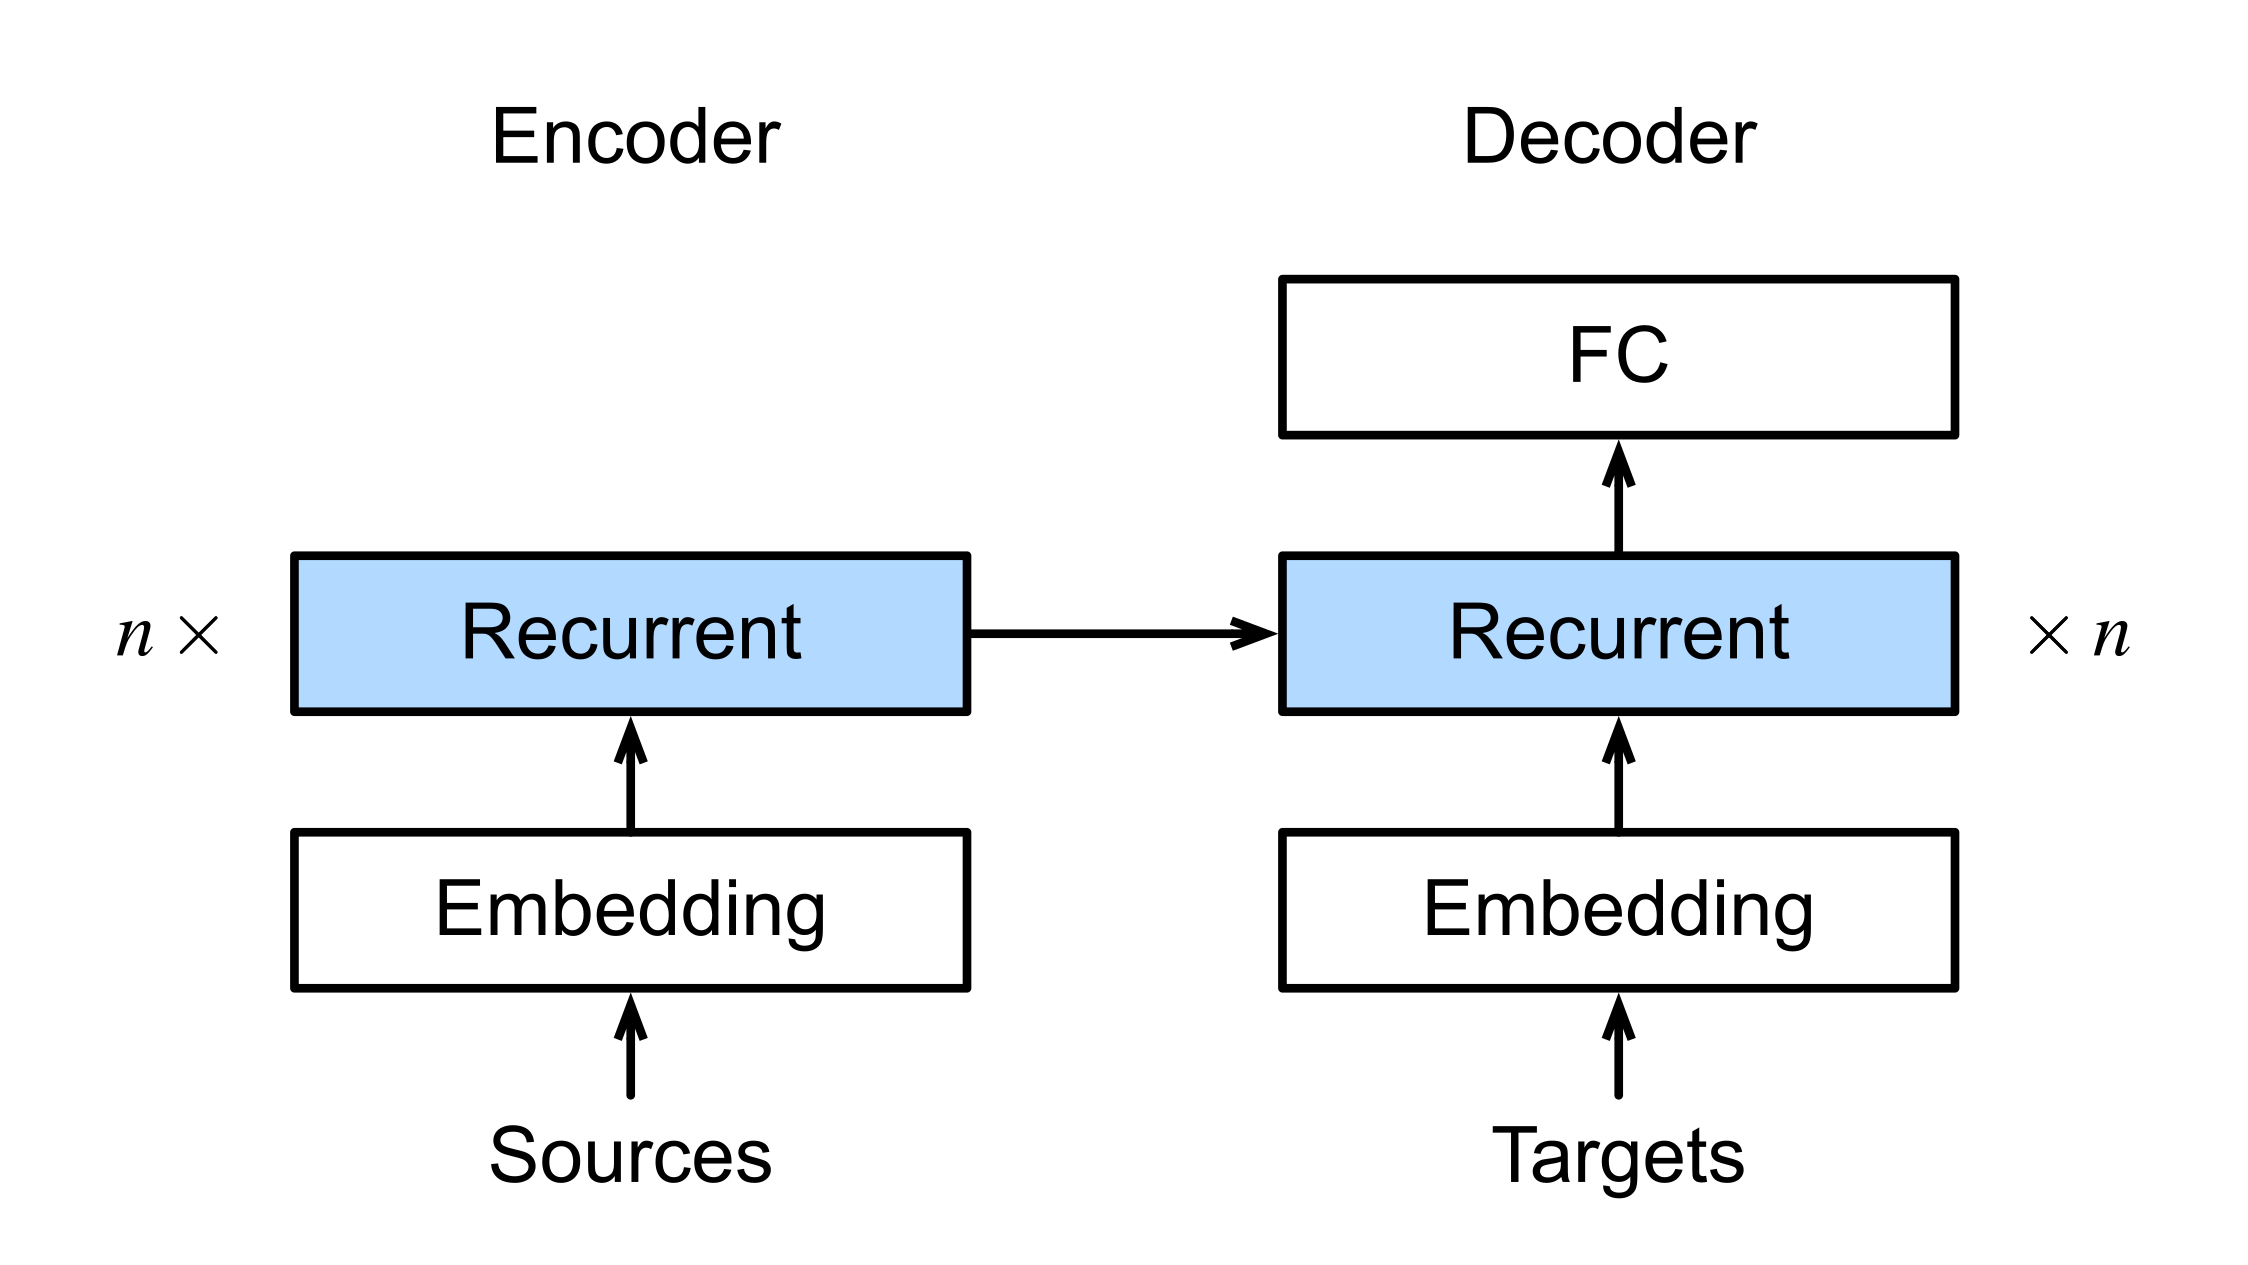
\includegraphics[scale = 0.1]{RNN-en-de.png}
\end{frame}

\section{Attention Prompt}
\begin{frame}
    \frametitle{Attention Prompt}
    A simple regression Problem: $f \in \{(x_1, y_1), (x_2, y_2), \ldots, (x_n, y_n)\}$.
    \begin{itemize}[label = \textbullet]
        \item Average Pooling: 
            \[f(x) = \frac{1}{n} \sum_{i=1}^n y_i\]
        \item Attention Pooling: 
            \[f(x) = \sum_{i=1}^n \alpha(x, x_i) y_i \]
    \end{itemize}
    We call $x$ a \emph{query} and $(x_i, y_i)$ a \emph{key-value} pair. \\
    $\alpha$ is the attention weight, which is the target.
    \footfullcite[]{D2l}
\end{frame}
\begin{frame}
    \frametitle{Attention Prompt}
    \begin{itemize}[label=\textbullet]
        \item Nonparametric: 
            \begin{align*}
                \alpha(x, x_i) &= \frac{K(x-x_i)}{\sum_{j} K(x-x_j)} \\
                K(u) &= \frac{1}{\sqrt{2\pi}} \exp \Bigl(-\frac{u^2}{2}\Bigr)
            \end{align*}
        \item parametric: learnable \emph{Attention Scoring Function}
    \end{itemize}
\end{frame}

\section{Transformer}
\begin{frame}
    \frametitle{Transformer}
    \begin{itemize}[label = \textbullet]
        \item Relys entirely on multi-head self-attention
        \item Encoder-Decoder architecture
        \item Positional encoding
    \end{itemize}
    \footfullcite[]{Attention}
\end{frame}

\subsection{Architecture}
\begin{frame}
    \frametitle{Architecture}
    \begin{columns}
        \begin{column}[]{0.5\textwidth}
            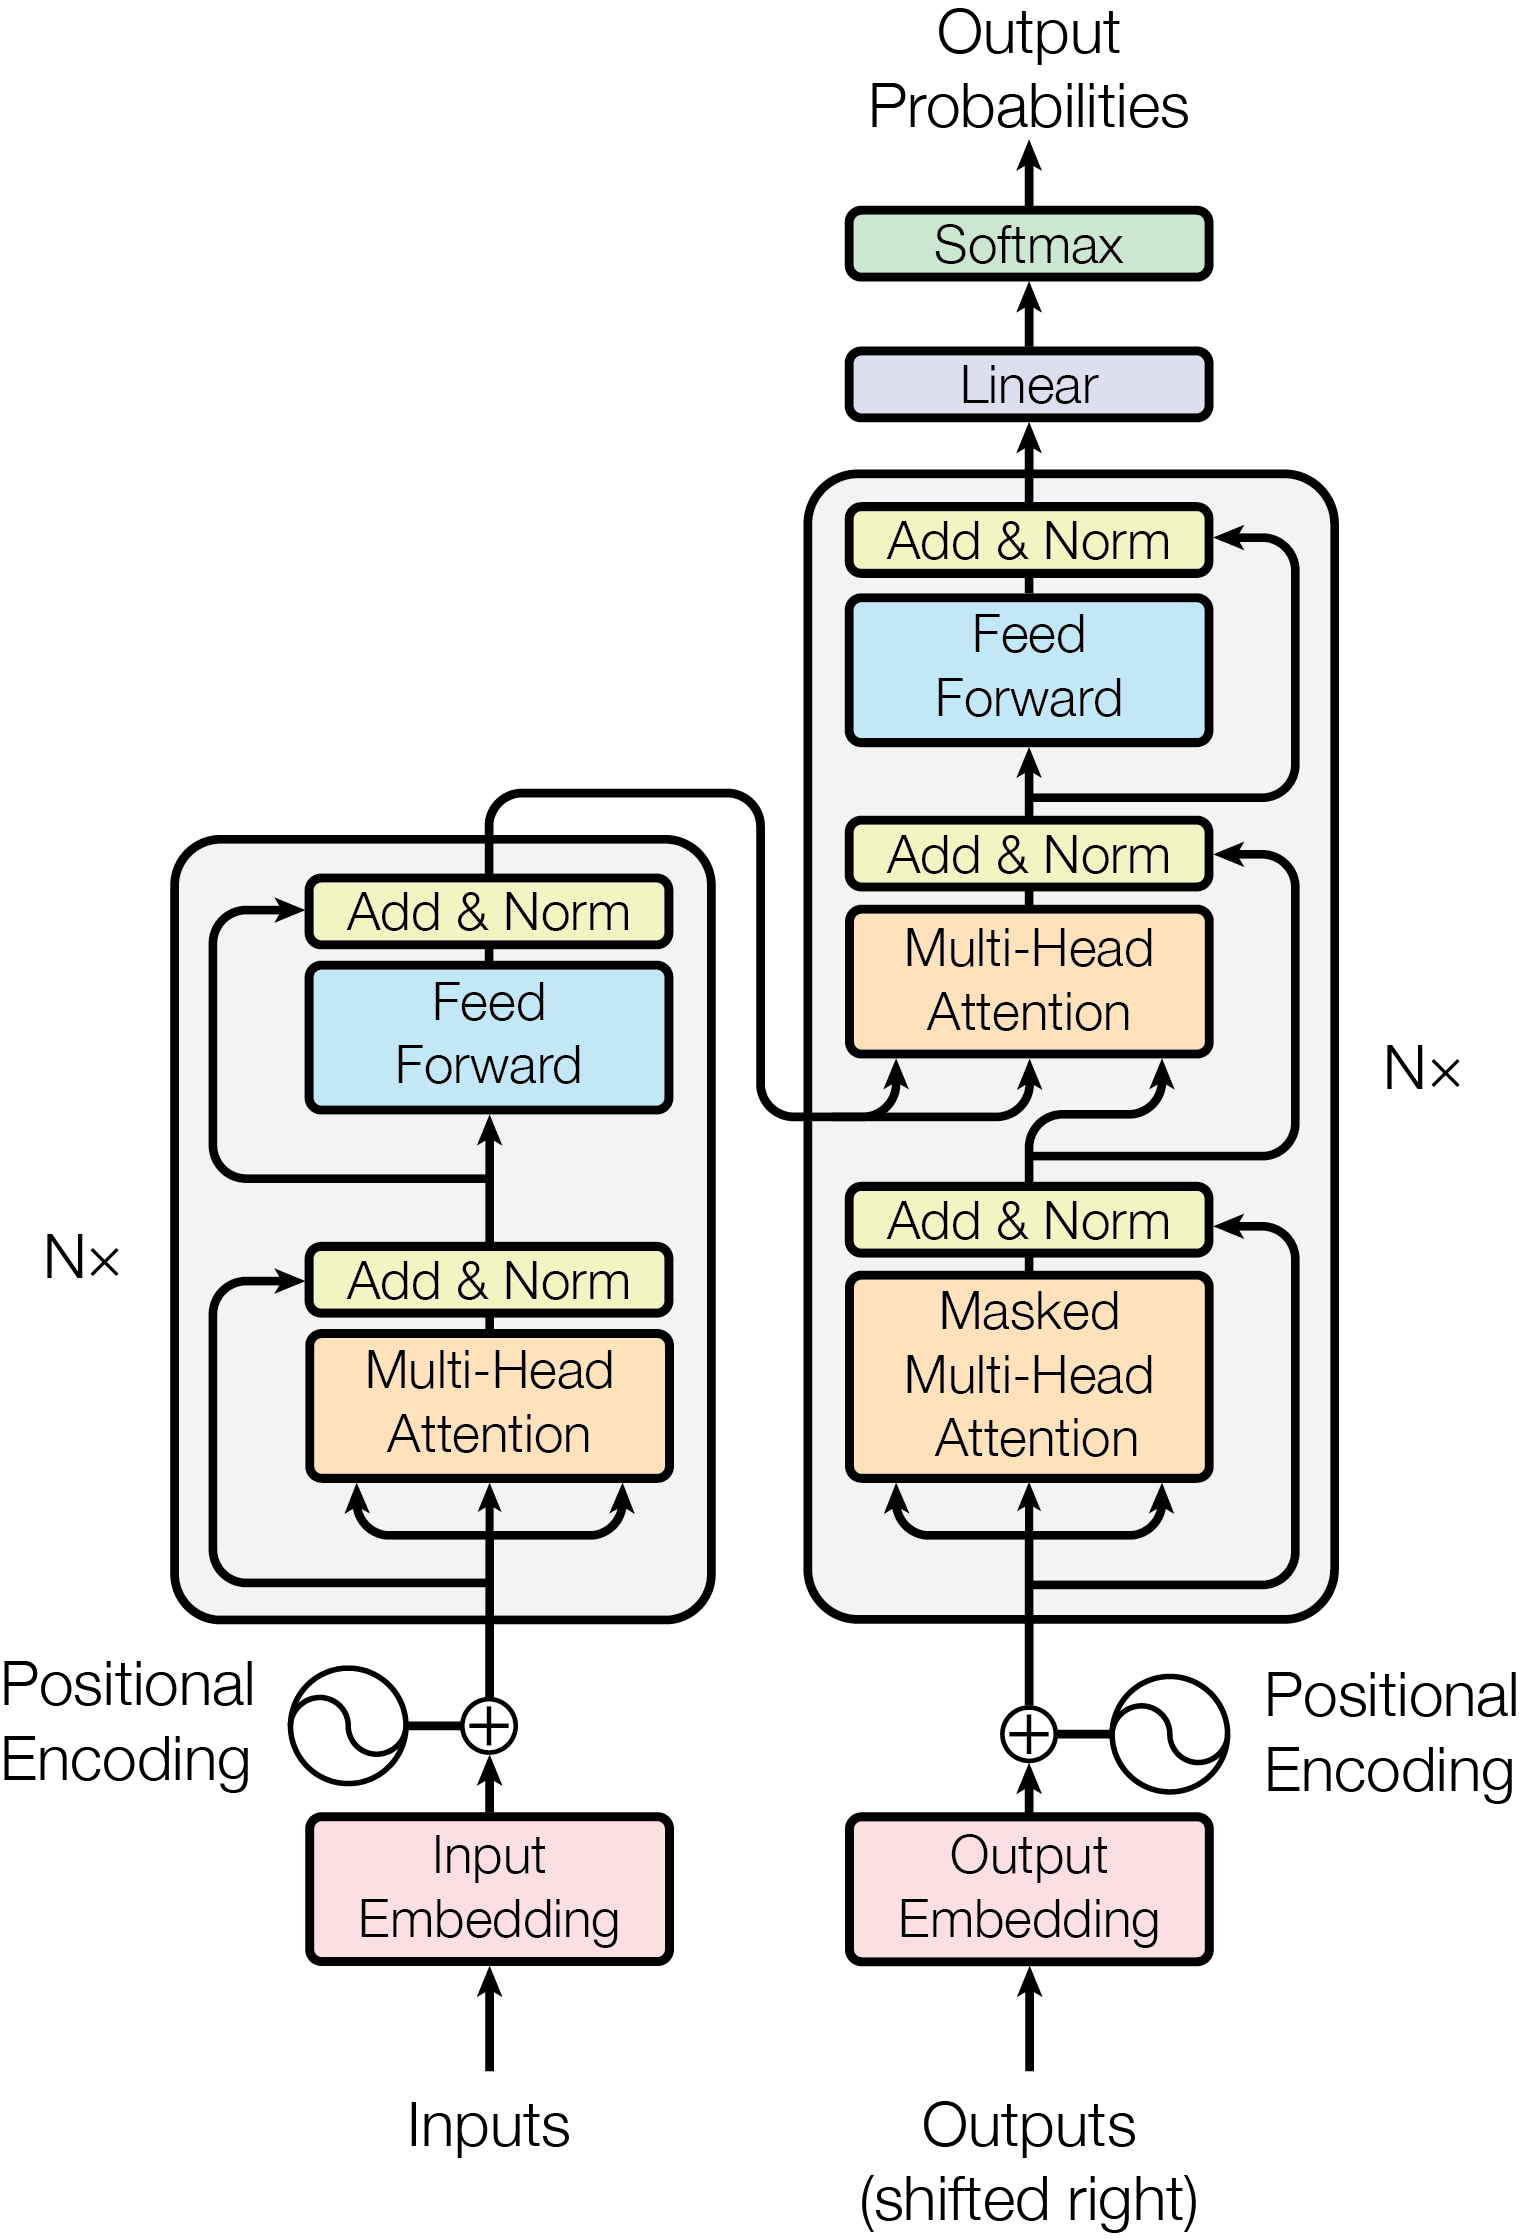
\includegraphics[scale = 0.4]{ModalNet-21.png}
        \end{column}
        \begin{column}{0.5\textwidth}
            \begin{itemize}
                \item 
                    Encoder: 
                    \begin{itemize}
                        \item $N = 6$ layers
                        \item Multi-head self-attention + feed forward
                    \end{itemize}
                \item Decoder: 
                    \begin{itemize}
                        \item Masked Multi-head self-attention
                        \item Multi-head attention
                    \end{itemize}
                \item Others:
                    \begin{itemize}
                        \item Positional Encoding
                        \item Layer-normalization
                    \end{itemize}
            \end{itemize}
                    
        \end{column}
    \end{columns}
\end{frame}

\subsection{Scoring Function}
\begin{frame}
    \frametitle{Scoring Function}
    Scaled Dot-Product Attention
    \begin{align*}
        Attention(Q, K, V) = \text{softmax} \Biggl(\frac{QK^T}{\sqrt{d_k}}\Biggr) V
    \end{align*}
    \begin{align*}
        Q \in \bb{R}^{n\x d_k}~~K \in \bb{R}^{m\x d_k}~~V\in \bb{R}^{m\x d_v}
    \end{align*}
\end{frame}

\subsection{Multi-Head Attention}
\begin{frame}
    \frametitle{Multi-Head Attention}
    It is beneficial to linearly project $Q, K, V$ to $d_k, d_k, d_v$ dimensions $h$ times.
    \begin{align*}
        Multihead(Q,K,V) &= Concat(head_1, \ldots, head_n) W^O \\
        \text{where}~head_i &= Attention(QW_i^Q, KW_i^K, VW_i^V)
    \end{align*}
\end{frame}

\subsection{Self-Attention}
\begin{frame}
    \frametitle{Self-Attention}
    Self-attention: 
    \begin{align*}
        \{f(x_i), 1 \le i \le n\}  \\
        \text{where}~f \in \{(x_i, x_i)\}
    \end{align*}
\end{frame}

\subsection{Positional Encoding}
\begin{frame}
    \frametitle{Positional Encoding}
    For $P \in \bb{R}^{n\x d}$:
    \begin{align*}
        p_{pos,2i} &= \sin \Bigl(\frac{i}{10000^{2i/d}}\Bigr) \\
        p_{pos,2i+1} &= \cos \Bigl(\frac{i}{10000^{2i/d}}\Bigr)
    \end{align*}
    $n$\: length of sequence; $d$\: length of encoding. \\
    Give each position-embedding pair a \emph{unique} value.
\end{frame}

\subsection{Recap}
\begin{frame}
    \frametitle{Recap}
    \begin{columns}
        \begin{column}[]{0.5\textwidth}
            \begin{figure}[r]
                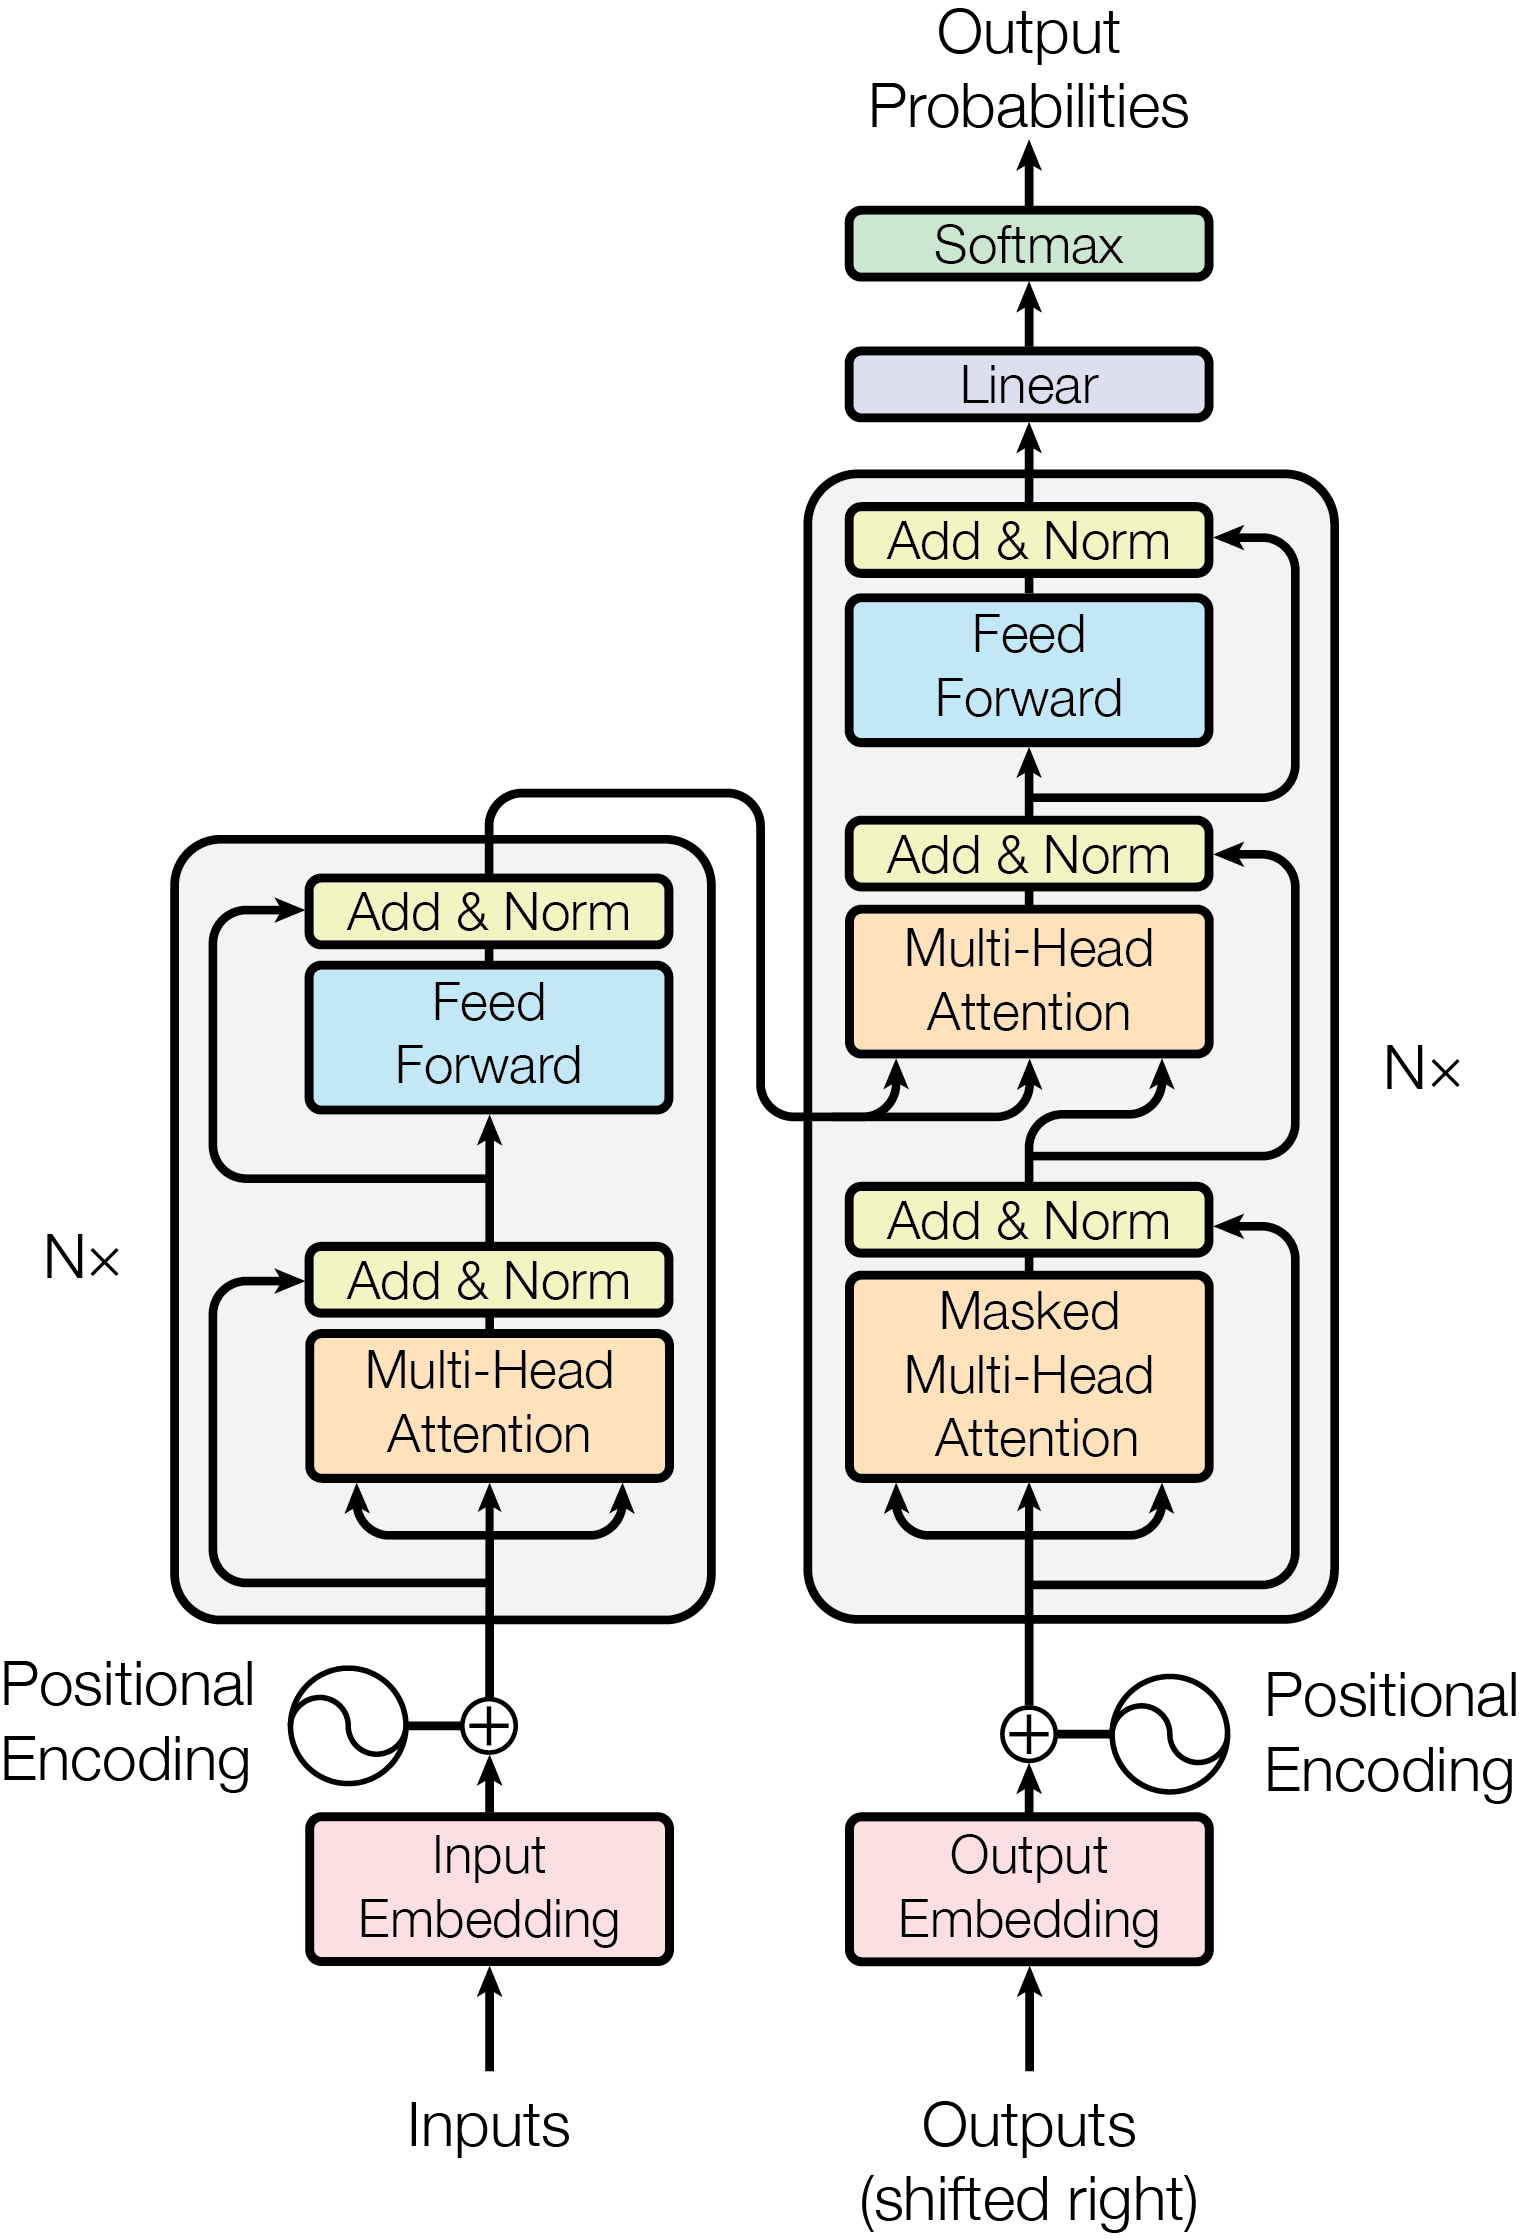
\includegraphics[scale = 0.4]{ModalNet-21.png}
            \end{figure}
        \end{column}
        \begin{column}[]{0.5\textwidth}
            \begin{figure}[r]
                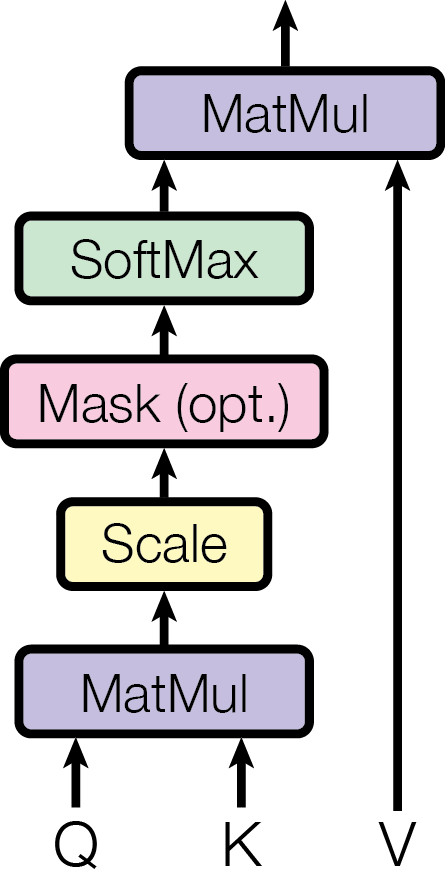
\includegraphics[scale = 0.6]{ModalNet-19.png}
            \end{figure}
        \end{column}
    \end{columns}    
\end{frame}

\section{VIT}
\begin{frame}
    \frametitle{VIT}
    \begin{itemize}
        \item VIT\: Vision Transformer
        \item Split images into fixed-size patches
    \end{itemize}
    \centering
    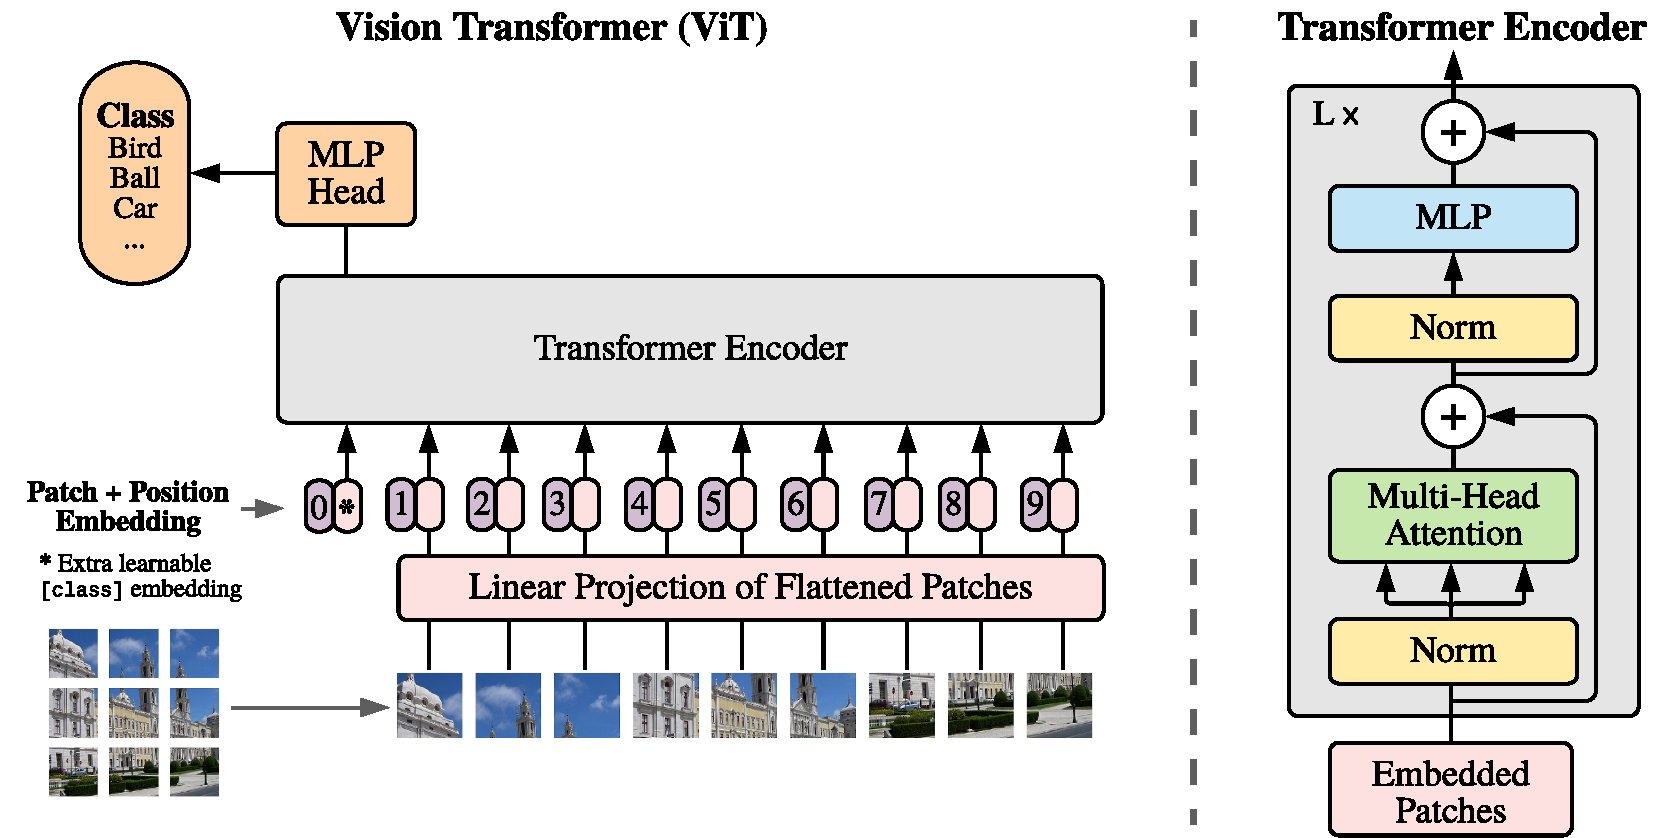
\includegraphics[scale = 0.4]{model_scheme.pdf}
    \footfullcite[]{VIT}
\end{frame}

\section{Medical-Related}

\subsection{Attention UNet}
\begin{frame}
    \frametitle{Attention UNet}
    \begin{figure}
        \centering
        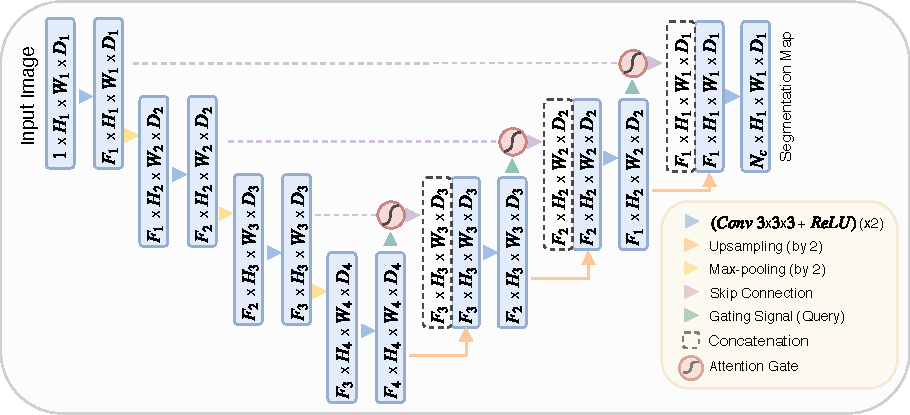
\includegraphics[scale = 0.7]{figure4.pdf}
    \end{figure}
    \begin{align*}
        Concat(Attention, upsample)
    \end{align*}
\end{frame}
\begin{frame}
    \frametitle{Attention Unet}
    \begin{figure}
        \centering
        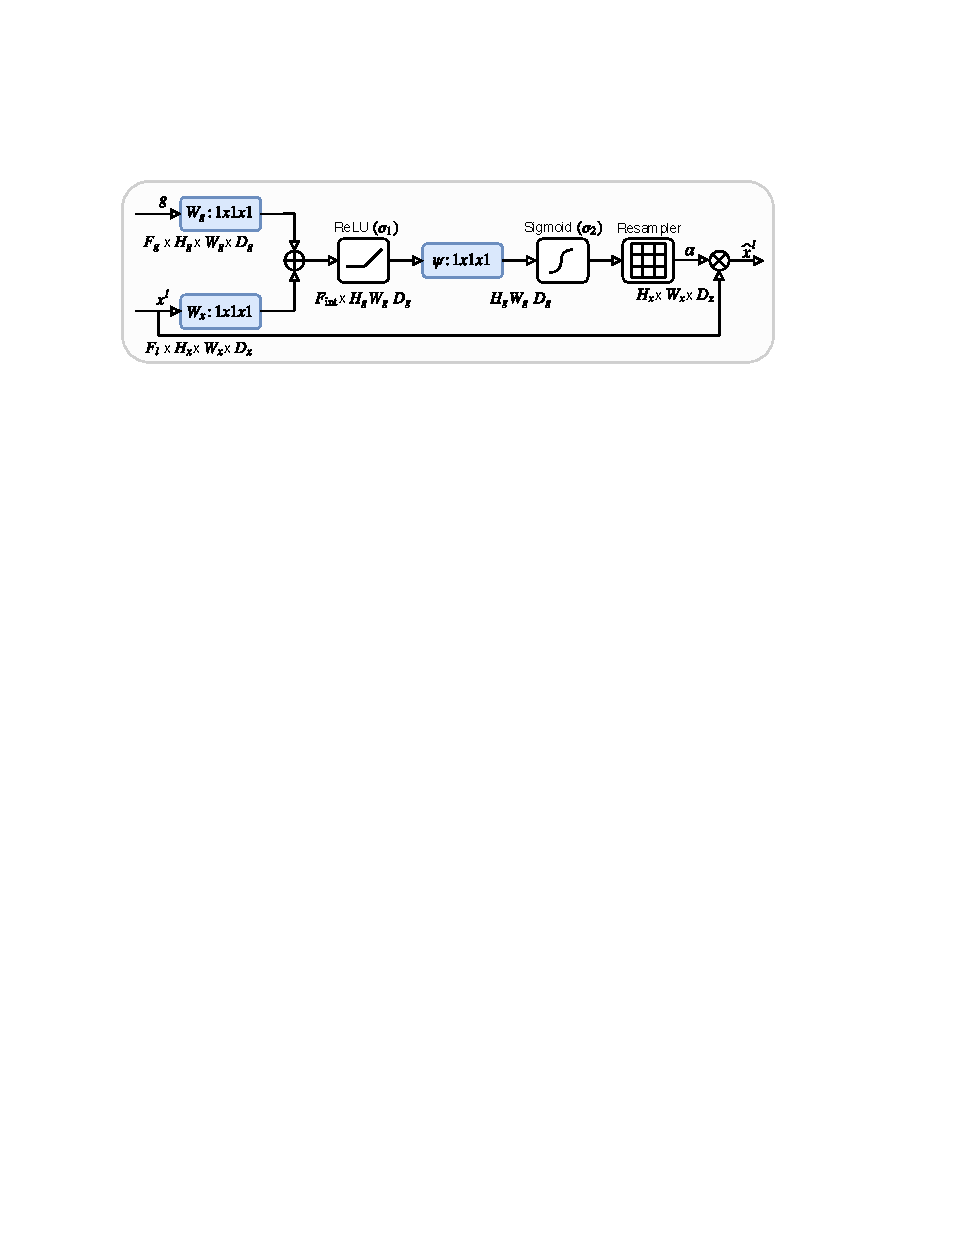
\includegraphics[scale = 0.9]{figure3.pdf}
    \end{figure}
    Using \emph{query $g$} from a coarser scale.
    Resampler\: Trilinear interpolation is applied.
    \footfullcite{UNet}
\end{frame}

\section{Conclusion}
\subsection{Inductive Bias}
\begin{frame}
    \frametitle{Inductive Bias}
    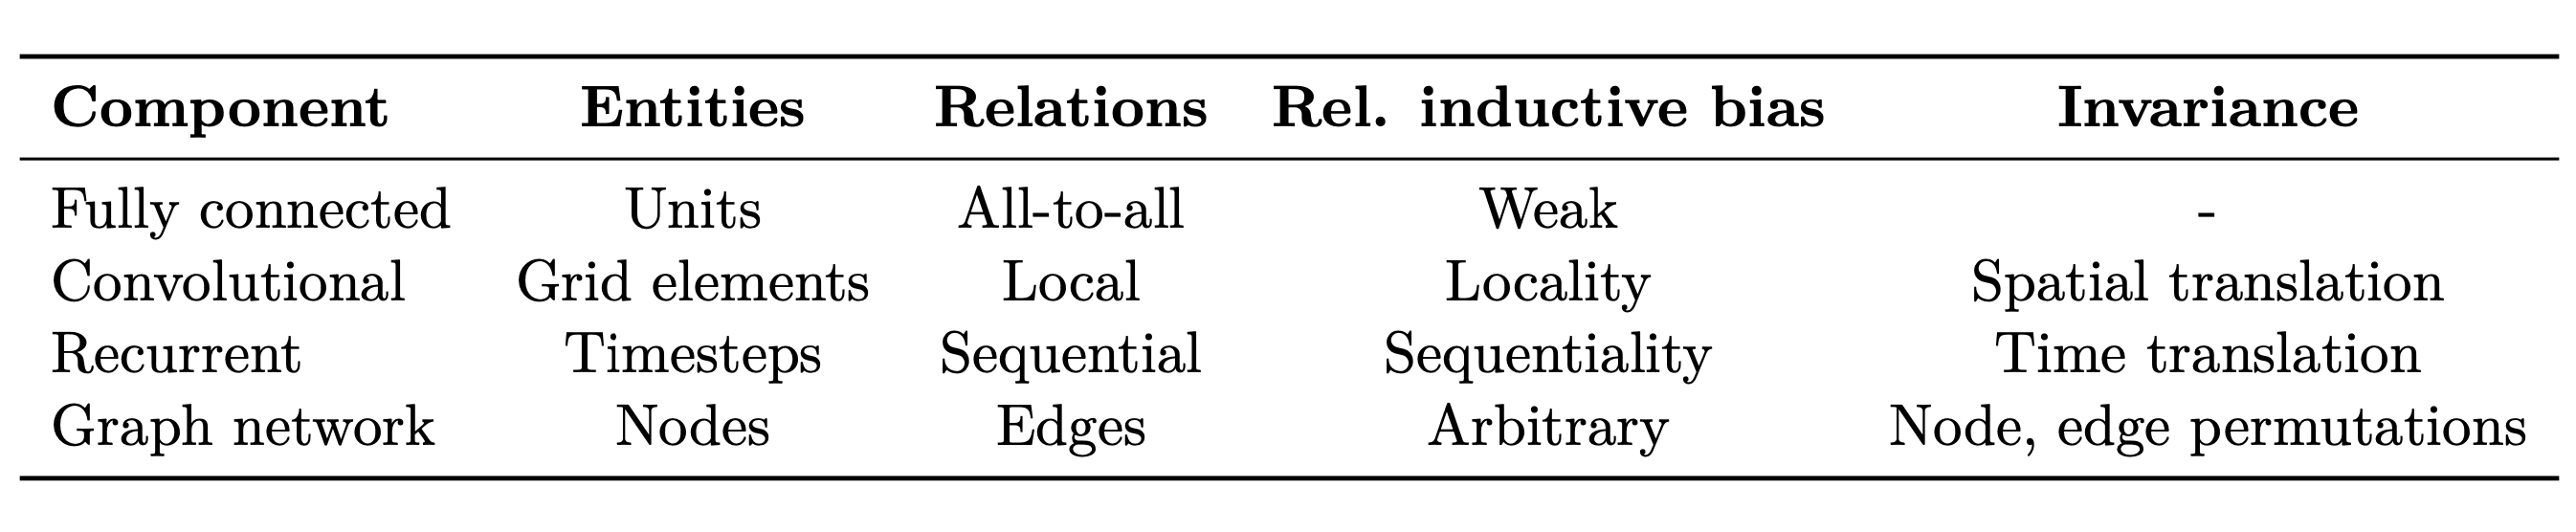
\includegraphics[scale = 0.25]{inductive-bias.png}
    \fullcite{GNN}
\end{frame}

\begin{frame}
    \printbibliography{}
\end{frame}

\end{document}